% $Log: abstract.tex,v $
% Revision 1.1  93/05/14  14:56:25  starflt
% Initial revision
% 
% Revision 1.1  90/05/04  10:41:01  lwvanels
% Initial revision
% 
%
%% The text of your abstract and nothing else (other than comments) goes here.
%% It will be single-spaced and the rest of the text that is supposed to go on
%% the abstract page will be generated by the abstractpage environment.  This
%% file should be \input (not \include 'd) from cover.tex.
\begin{figure}[ht]
\centering
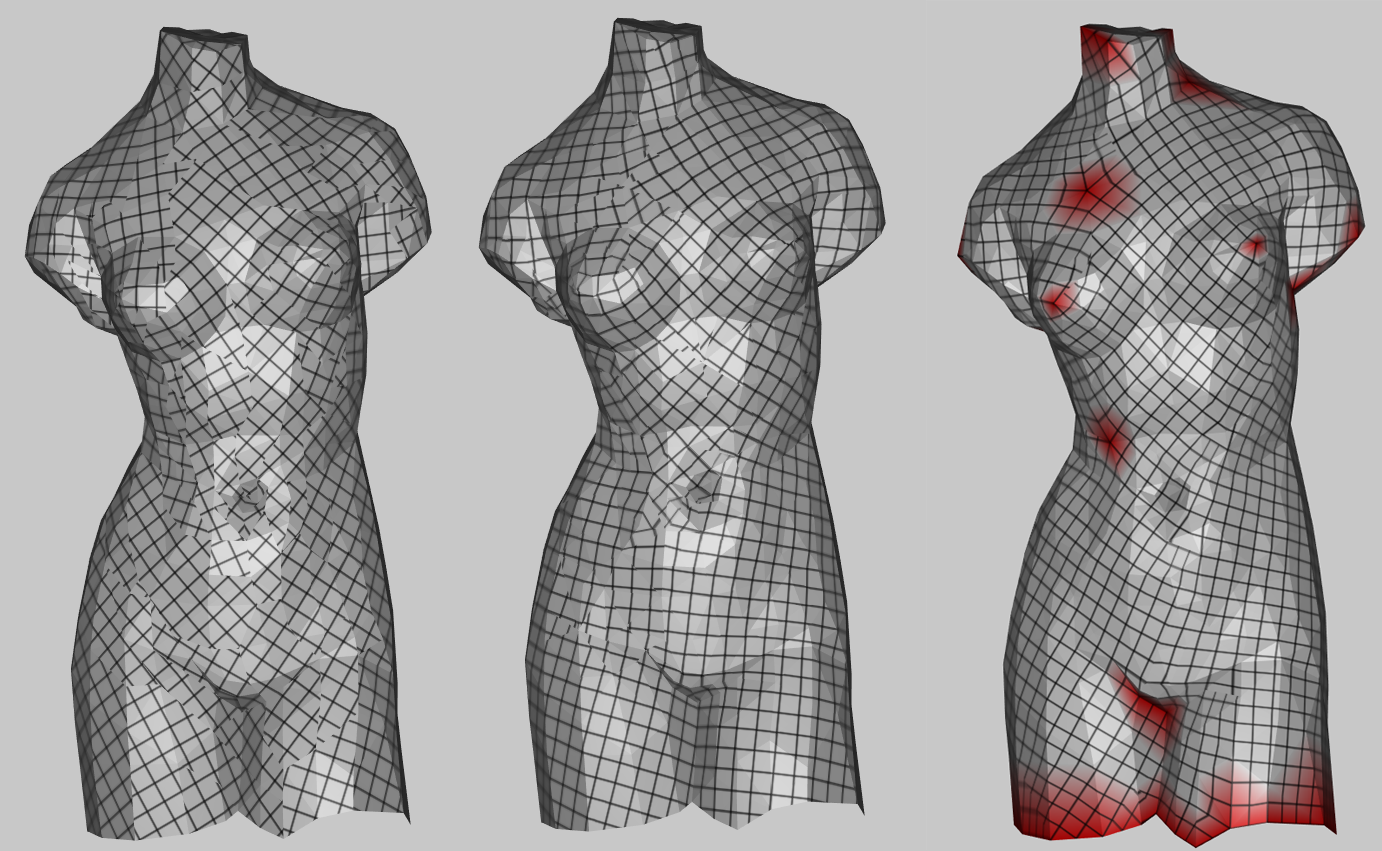
\includegraphics[width=15cm]{figures/teaser.png}
\caption[Abstract's Teaser]{\textbf{Left:} Initial mapping of cut mesh. \textbf{Middle:} With increased penalty on seamlessness violation. \textbf{Right:} With increased penalty on integer violation.}
\label{fig:teaser}
\end{figure}

\subsubsection{Introduction}
Many applications in computer graphics, such as character modeling and animation, architectural geometry, and also physical simulation to some extent, call for quad meshes as a representation of the geometry \cite{10.1111/cgf.12014}. However, since triangle meshes are generally more prevalent, they need to be convert via the process known as \emph{quad remeshing}.

\noindent Numerous techniques were introduced in recent years, and the most common approach is to split the problem into cross field generation, and field guided parameterization. In this document, we present an interactive, direct parametrization approach, which nullifies the need for intermediate steps.

\noindent The idea behind parameterization based methods in general, is to map the mesh to the plane, and create a regular grid layout on it. In order to ensure that the grid on the plane is transformed into a valid quad mesh on the surface, certain conditions on the parameterization must be fulfilled \cite{bommes:hal-00862648}:

\begin{enumerate}
  \item \textbf{Seamless Condition}: The transition function $g_{ij}$ between two half-edges $e_i$ and $e_j$ on the parameterization domain that corresponds to the same surface edge that is part of a cut seam, has to be an integer-grid automorphism given by:
  $$e_j = R^{r_{ij}}_{90^\circ}e_i + \vec{t}_{ij}$$
  Where  $r_{ij} \in \{0,1,2,3\}$ and $\vec{t}_{ij} \in \mathbb{Z}^2$.
  
  \item \textbf{Singular-Points Condition}: All singular vertices, which are characterized by a non-zero angular defect on the parameterization domain, have to lie on integer locations. That is, given the set $S_i$ of all parameterization domain vertices that correspond to the same singular surface vertex $v_i$, we require that:
  $$\forall u \in S_i: u \in \mathbb{Z}^2 $$
  
  \item \textbf{Consistent Orientation Condition}: All triangles on the parameterization domain should have the same orientation. That is, we should not allow triangle flips after initial mapping is formed.
\end{enumerate}

\subsubsection{Our Approach}
Inspired by \cite{Poranne:Autocuts:2017}, we employ a direct approach to the problem of quadrangulating a triangle mesh, by formulating and solving a smooth optimization problem. We model smooth penalty functions for the first two conditions mentioned above (Seamless and Singular-Points), and add to it an additional penalty, the Symmetric Dirichlet energy, which prevents triangle flips and penalize triangle distortion.
Since all of our penalty functions are smooth, we can analytically derive their gradients and hessians, and utilize Newton's method to iteratively solve for a mapping that renders a valid quad mesh on the 3D surface.

\noindent Our smooth approach allows us to visualize the whole optimization process for the end-user as an interactive design tool, which empowers the user to guide the algorithm to the desired result by gradually changing penalty weights, grid resolution, guiding quads direction using brush tool, and more. The user receives immediate feedback for any change applied to the problem settings. Figure \ref{fig:teaser} illustrates the three main stages of our approach. First, the 3D surface is cut into the plane. Then, the seamless penalty function weight gradually increased. Finally, the singular points penalty function is turned on to place singular vertices at integer locations.

\subsubsection{Details}
\paragraph{Initialization}
We cut the input triangle-mesh open by isometrically mapping its dual spanning tree to the parameterization plane as a triangle-soup. We first map an arbitrary initial triangle to the parameterization plane. Next, we map to the plane all adjacent triangles of the initial triangle, such that adjacent triangles on the mesh surface share an edge on the 2D domain. We continue this process for the next layer of neighbours, till we map the whole input mesh.
\subsubsection{Seamless Penalty Functions}
\paragraph{Angle Penalty}
Given two half-edges $e_i$ and $e_j$ on the parameterization domain that corresponds to the same surface edge, we penalize the angle between them as follows: 
\begin{flalign}
P_{\mathrm{angle}}\left(e_i,e_j\right) = \sin\left(4\left(\theta(e_i) - \theta(e_j) \right) - \frac{\pi}{2} \right) + 1
\end{flalign}
Where $\theta(e_i)$ and $\theta(e_j)$ are the angles of the two half edges $e_i$ and $e_j$ with respect to the horizontal Cartesian isolines, respectively. For any $k \in \mathbb{Z}$ such that $\theta(e_i) - \theta(e_j) = \frac{\pi}{2}k$ we have that $P_{\mathrm{angle}}\left(e_i,e_j\right) = 0$. Therefore, $P_{\mathrm{angle}}$ will penalize half-edges of which their angle discrepancy differs from a multiple of $90^\circ$.
\paragraph{Length Penalty}
We penalize the length discrepancy between the two half-edges with the following penalty function:
\begin{flalign}
P_{\mathrm{length}}\left(e_i,e_j\right) = \left( \norm{e_i}^2 - \norm{e_j}^2 \right)^2
\end{flalign}
Only when the two half-edges have the same length, we have that $P_{\mathrm{length}}\left(e_i,e_j\right) = 0$.
\paragraph{Translation Penalty}
We penalize for non-integer translation between the two half-edges as follows:
\begin{flalign}
P_{\mathrm{translation}}\left(e_i,e_j\right) &= \sin\left(2\pi\left(x_{e_i} - x_{e_j}\right) - \frac{\pi}{2} \right) + 1 \\ & \quad + \sin\left(2\pi\left(y_{e_i} - y_{e_j}\right) - \frac{\pi}{2} \right) + 1 \notag
\end{flalign}
Where $\left(x_{e_i}, y_{e_i}\right)$ and $\left(x_{e_j}, y_{e_j}\right)$ are the coordinates of two twin-vertices of the two half-edges $e_i$ and $e_j$.
\subsubsection{Singular-Points Penalty Function}
To satisfy the singular-points condition, all twin-vertices on the parameterization domain have to lie on integer locations, if they correspond to a singular-points on the mesh surface. Therefore, we penalize singular points as follows:
\begin{flalign}
P_{\mathrm{singular}}\left(S\right) = \sum_{v \in S} \left( \sin\left(2 \pi x_{v} - \frac{\pi}{2} \right) + 1 + \sin\left(2 \pi y_{v} - \frac{\pi}{2} \right) + 1 \right)
\end{flalign}
Where $S$ is a set of domain twin-vertices that correspond to a singular-point, and $\left(x_v,y_v\right)$ are the coordinates of domain vertex $v \in S$.
\subsubsection{Consistent Orientation and Distortion Penalty Functions}
To satisfy the consistent orientation condition, and to minimize triangle distortion, we use the symmetric dirichlet energy \cite{Smith:2015}, which prevents triangle flips and promotes isometric mappings. The symmetric dirichlet penalty function is given as follows:
\begin{flalign}
P_{\mathrm{dirichlet}}\left(t_i\right) = \norm{J\left(t_i\right)}_F^2 + \norm{J^{-1}\left(t_i\right)}_F^2
\end{flalign}
Where $J\left(t_i\right)$ is the Jacobian of the mapping of triangle $t_i$ and $\norm{\cdot}_F$ is the Frobenius norm.
\subsubsection{Optimization Process}
In order to find a parameterization which forms a valid quad mesh on the 3D surface, we solve the following unconstrained optimization problem:
\begin{flalign}
\min_{X} & \quad \sum_{i \sim j} \Big( P_{\mathrm{angle}}\left(e_i,e_j\right) + P_{\mathrm{length}}\left(e_i,e_j\right) + P_{\mathrm{translation}}\left(e_i,e_j\right) \Big) \\
 & + \sum_{i} P_{\mathrm{singular}}\left(S_i\right) \notag \\
 & + \sum_{i} P_{\mathrm{dirichlet}}\left(t_i\right) \notag
\end{flalign}
Where $X$ denotes the set of variables of the optimization problem, i.e., the coordinates of the vertices in the parameterization domain. We derive analytical expressions for the gradient and Hessian of each penalty function, and modify the computed Hessians to be positive-definite if necessary (by using singular-value decomposition and eliminating negative singular values). We solve the optimization problem using Newton's method. In iteration $i$, we evaluate the gradient $g^{(i)}$ and Hessian $H^{(i)}$ of our total objective function at $X^{(i)}$, and solve the Newton equation $H^{(i)}d^{(i)}=-g^{(i)}$ which yields a search direction $d^{(n)}$. The next iterate is obtained by $X^{(i+1)} = X^{(i)} + \alpha p^{(i)}$ where the optimal $\alpha$ is found using line search. We use Intel's MKL PARDISO solver to solve the sparse linear system of equations induced by the Newton's method.
